%% CISR conference submission version, adapted from the Springer Nature version
%% Template: IEEEtran.cls (conference mode); reference style: IEEEtran.bst
%% Compile: pdflatex main.tex && bibtex main && pdflatex main.tex && pdflatex main.tex
\documentclass[conference]{IEEEtran}
\IEEEoverridecommandlockouts

\usepackage{cite}
\usepackage{amsmath,amssymb,amsfonts}
\usepackage{graphicx}
\usepackage{textcomp}
\usepackage{xcolor}
\usepackage{booktabs}   % \bottomrule used in tables
\usepackage{multirow}
\usepackage{algorithm}
\usepackage{algpseudocode}
\usepackage{url}

\begin{document}

\title{Latency Optimization of Cascaded Voice Dialogue Systems with a Pipeline-Parallel Streaming Architecture\thanks{Corresponding author: Zhengyou Liang (zhyliang@gxu.edu.cn).}}

% Authors: all listed in IEEE conference author-block format, with numbered affiliation.
\author{\IEEEauthorblockN{1\textsuperscript{st} Haihua Mo}
\IEEEauthorblockA{\textit{School of Computer, Electronics} \\
\textit{and Information, Guangxi University}\\
Nanning, China \\
hua0424@163.com}
\and
\IEEEauthorblockN{2\textsuperscript{nd} Zhengyou Liang}
\IEEEauthorblockA{\textit{School of Computer, Electronics} \\
\textit{and Information, Guangxi University}\\
Nanning, China \\
zhyliang@gxu.edu.cn}
}

\maketitle

\begin{abstract}
Cascaded ASR--LLM--TTS dialogue systems preserve modularity but leave speech recognition and prompt prefilling on the post-utterance critical path. We present a pipeline-parallel architecture that overlaps chunked Whisper recognition with incremental LLM prefilling. Silero VAD and a timestamp-aligned sliding window produce an append-only downstream transcript stream, while a reusable key--value cache moves most prompt processing into the user's speaking time. We evaluate 1,132 synthesized MultiWOZ/CrossWOZ utterances, concatenated human-read speech from LibriSpeech and AISHELL-1, a matched LocalAgreement-2-style baseline, and a unified time-to-first-audio (TTFA) path. On the same 498-sample synthetic subset, the overall TTFT reduction is 74.3\% on the original platform and 70.4\% on a second dual-RTX~3090 platform. For Extra Long human-read speech, reductions are 67.5\% on LibriSpeech and 65.7\% on AISHELL-1. Streaming ASR accounts for most of the measured gain; incremental prefilling has a smaller independent effect under Qwen2-7B. Unified-timeline measurements reduce median TTFA from 22.27~s to 3.11~s, although TTS remains a variable bottleneck. Internal ASR hypotheses can still drift after commitment, but no downstream rollback is issued; an exploratory 50-sample semantic evaluation reports a mean response-embedding cosine of 0.883.
\end{abstract}

\begin{IEEEkeywords}
intelligent systems, human--computer interaction, voice dialogue system, streaming architecture, pipeline parallelism, incremental prefilling, end-to-end latency
\end{IEEEkeywords}

\section{Introduction}\label{sec:intro}

Spoken language interfaces have become a core modality of intelligent systems and human--computer interaction, spanning service robots, intelligent transportation, and smart assistants. Within this trend, human--computer interaction is evolving from command-style input toward natural spoken dialogue. Although multimodal large models such as GPT-4o and Gemini 1.5 have advanced voice interaction capabilities, constraints on deployment cost and engineering maturity mean that most production systems still adopt a cascaded architecture composed of automatic speech recognition (ASR), a large language model (LLM), and text-to-speech (TTS). For long-form speech, this architecture typically waits for endpoint detection to complete before starting downstream understanding and generation, which introduces post-endpoint waiting latency and degrades the responsiveness and fluency of the interaction.

At the same time, voice dialogue systems built on large language models understand user intent better, handle complex reasoning, and support emotionally expressive multi-turn interaction. This higher level of intelligence, however, comes with substantial computational overhead and latency challenges. Published system reports indicate that GPT-4o achieves an end-to-end voice response latency as low as 232~ms, with an average of 320~ms~\cite{ref1}, already approaching human conversational reaction speed. Low latency has therefore become, alongside accuracy, a key competitive metric for the next generation of voice interaction.

Although end-to-end multimodal models perform impressively in papers and experiments, they are expensive to train, complicate data-privacy governance, and require deep customization for vertical scenarios. A cascaded system instead decomposes the pipeline into independent, replaceable modules---voice activity detection (VAD)~\cite{ref2}, ASR, an LLM, and TTS---connected in sequence, and can thus reuse existing high-quality ASR, text LLM, and TTS capabilities. In scenarios that require rapid LLM iteration, controlled deployment cost, and low upgrade risk, the cascaded architecture retains substantial engineering value. In such a serial architecture, the total system latency ($T_{\mathrm{total}}$) depends not only on the processing time of each module but also, to a significant degree, on how data flows between modules. For analysis, we express the total latency of a serial cascaded system as a simple linear sum of the component latencies:
\begin{align}
T_{\mathrm{total}} ={}& T_{\mathrm{VAD}} + T_{\mathrm{ASR}} + T_{\mathrm{Prefill}} + T_{\mathrm{Decode}} \nonumber\\
& + T_{\mathrm{TTS}} + T_{\mathrm{Net}}
\label{eq:total}
\end{align}

Here $T_{\mathrm{VAD}}$ denotes voice-activity and turn-boundary processing, $T_{\mathrm{ASR}}$ speech recognition, $T_{\mathrm{Prefill}}$ prompt prefilling, $T_{\mathrm{Decode}}$ autoregressive decoding, $T_{\mathrm{TTS}}$ speech synthesis, and $T_{\mathrm{Net}}$ communication and serialization. Component overlap means that Eq.~(\ref{eq:total}) is a conceptual serial budget rather than an identity for the proposed pipeline. We therefore report two timestamp-defined metrics. Time to first token is
\begin{equation}
\mathrm{TTFT}=t_{\mathrm{first\ token}}-t_{\mathrm{speech\ end}},
\label{eq:ttft}
\end{equation}
and time to first audio is
\begin{equation}
\mathrm{TTFA}=t_{\mathrm{first\ playable\ PCM}}-t_{\mathrm{speech\ end}}.
\label{eq:ttfa}
\end{equation}
For the prerecorded legacy experiments, speech end is operationalized as completion of feeding the waveform. TTFT includes pipeline closure, remaining ASR and prefill work, and first-token selection, but excludes TTS. TTFA additionally includes response-text readiness, the local TTS request, and initial synthesis until at least 1324 bytes of non-empty playable PCM are available. The prototype uses in-process queues for ASR/LLM communication and a localhost TTS service, so it does not measure a distributed network path.

In conventional serial cascades, several seconds may elapse between speech end and spoken output. For long-form input, full-audio ASR and one-shot LLM prefilling both remain after speech end. As spoken interfaces enter service robots and conversational assistants, reducing this residual critical path is important for usability. The question addressed here is whether a modular cascade can move recognition and prefill work into the user's speaking interval without changing the underlying ASR and LLM weights.

\section{Related Work}\label{sec:related}

\subsection{Streaming Progress in Automatic Speech Recognition}

The processing speed of the ASR system determines how quickly user speech becomes text the LLM can consume. Early streaming ASR architectures were dominated by the RNN-Transducer (RNN-T)~\cite{ref3}. The recurrent nature of RNNs suits streaming audio well, but the step-by-step recurrent dependency limits parallelism over the time dimension during training and makes long-range semantic modeling difficult. With the advent of the Transformer, attention-based models pushed recognition accuracy to new levels~\cite{ref4}. However, the Transformer's global attention requires the entire input before computation can begin, so the vanilla Transformer cannot operate in a streaming fashion.

To address this, Google proposed the Conformer architecture, which combines the local feature extraction of convolutional neural networks (CNNs) with the global modeling of the Transformer and quickly became mainstream in industry~\cite{ref5}. In practice, streaming ASR often uses chunked processing with overlapped stitching: audio is segmented and recognized with a sliding window, and outputs are made consistent across overlap regions, balancing accuracy against latency. Whisper, for example, is an encoder--decoder model aimed primarily at offline transcription~\cite{ref6}; efforts to make such offline models streamable either modify the architecture---converting the non-causal encoder into a causal one so that smaller chunks can be transcribed online at lower latency---or modify the training objective, using sequence-level regularization to encourage earlier token emission and shorten the output lag of streaming recognition.

\subsection{LLM Inference Acceleration}

Once ASR transcription completes, LLM inference speed becomes the second major latency bottleneck, constrained mainly by the autoregressive generation of the Transformer decoder and by GPU memory bandwidth~\cite{ref7}. The key--value cache (KV cache) was introduced precisely to eliminate repeated computation during inference. By caching the Key/Value vectors of historical tokens, the model no longer recomputes intermediate results over the full context when generating a new token, reducing per-step decoding complexity from quadratic to linear in sequence length. The KV cache is now standard in modern inference engines such as vLLM and TGI~\cite{ref8}. For the prefill stage over long inputs, FlashAttention restructures GPU memory access with a tiled computation strategy, raising long-sequence throughput substantially and partially addressing the rapid growth of attention computation with sequence length~\cite{ref9}. For long conversations, StreamingLLM introduces an ``attention sink'' mechanism that anchors early tokens as fixed reference points, mitigating the degradation caused by context-window overflow and allowing the LLM to keep streaming stably within a bounded KV cache.

\subsection{Full-Pipeline Optimization of Voice Dialogue Systems}

Beyond optimizing ASR or the LLM in isolation, coordinated scheduling across the whole pipeline also matters for overall latency. In speech processing tasks such as speech translation, cascaded designs have long been a standard system paradigm: they reuse mature components and allow flexible module replacement, but they also incur intermediate-representation loss, error propagation, and accumulated inter-module latency~\cite{ref10}. Recent end-to-end streaming spoken dialogue models attempt to bypass the traditional ASR--LLM--TTS serial chain, pursuing lower interaction latency through speech-native modeling and streaming generation~\cite{ref11}. Open-source systems such as Mini-Omni, Moshi, and LLaMA-Omni fall into this line of exploration.

\subsection{Contributions of This Work}

\begin{figure*}[!t]
\centering
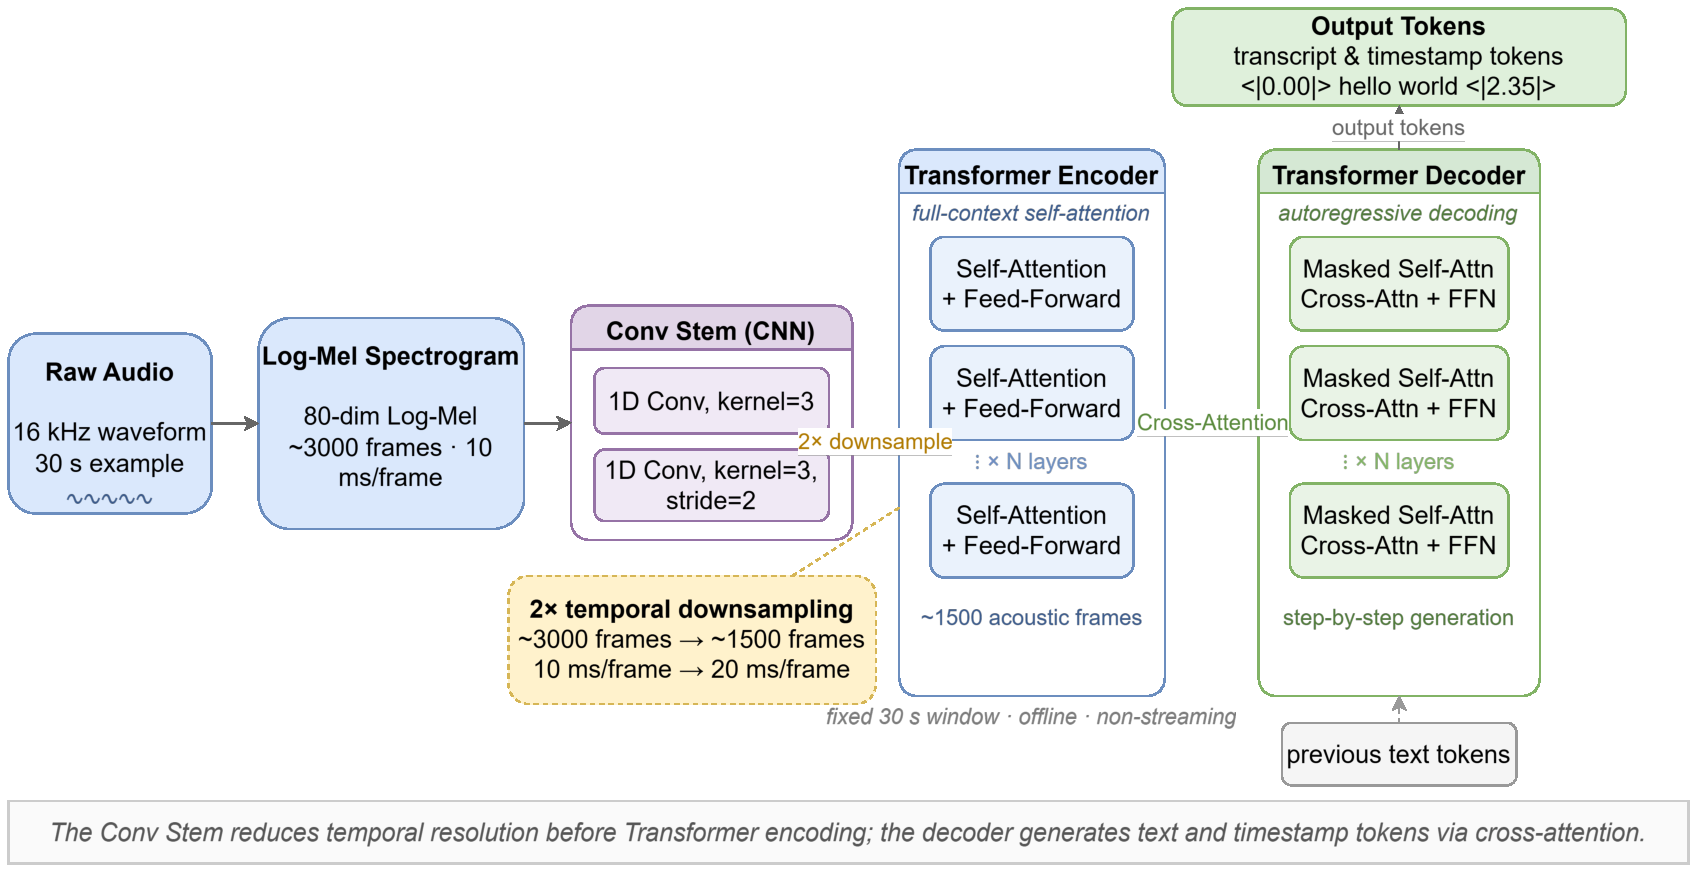
\includegraphics[width=\textwidth]{Fig1.pdf}
\caption{Overall architecture of the Whisper model and schematic of feature downsampling}
\label{fig:whisper}
\end{figure*}

When a traditional cascaded voice dialogue system processes long speech, per-module latencies accumulate stage by stage while computing resources sit idle. Existing work either optimizes the ASR model alone or extends the LLM into a multimodal architecture that generates speech directly; neither can reuse existing state-of-the-art text models. This paper proposes a fine-grained pipeline-parallel design (hereafter System~B) that is directly compatible with existing non-streaming ASR models and text LLMs. Our main contributions are:

\begin{itemize}
\item \textbf{Streaming ASR context management.} An adaptive Whisper sliding window combines Silero VAD, dynamic buffering, prefix--suffix acoustic context, and timestamp-aligned commitment to produce an append-only downstream text stream.

\item \textbf{Incremental LLM prefilling.} Newly committed fragments are prefetched into the LLM's KV cache during speech. Historical cached states are reused, relocating prompt computation into the input interval rather than claiming a lower asymptotic complexity.

\item \textbf{Broader latency and robustness evaluation.} In addition to the synthesized MultiWOZ/CrossWOZ benchmark, we evaluate concatenated LibriSpeech/AISHELL-1 human-read speech, noise and speed perturbations, repeated measurements, a matched LocalAgreement-2-style baseline~\cite{machacek2023turning,liu2020partialhypothesis}, and first-audible-output latency.

\item \textbf{State-correctness and downstream analysis.} We measure internal ASR drift, tokenizer seams, and response-level semantic consistency, distinguishing the append-only downstream contract from stronger and unsupported claims of internal hypothesis or KV-state equivalence.
\end{itemize}

\section{Principles and Methods}\label{sec:methods}

\subsection{Automatic Speech Recognition}

\subsubsection{Whisper Architecture and Its Offline Nature}

We adopt OpenAI's Whisper as the speech-to-text module. Whisper is an end-to-end Transformer encoder--decoder model that outputs text tokens directly from speech features. Pretrained on large-scale weakly supervised speech--text data, it is robust across languages, accents, and noise conditions~\cite{ref12}.

As shown in Fig.~\ref{fig:whisper}, Whisper converts 16~kHz audio into 128-dimensional log-Mel spectrogram features (consistent with the Whisper-Turbo, i.e., large-v3-turbo, model used in our experiments; earlier Whisper models use 80 dimensions), downsamples them through a convolutional front end, and feeds them to a Transformer encoder; the decoder reads the encoder representations through cross-attention and autoregressively emits text tokens. Its vocabulary includes timestamp tokens that provide segment- or word-level alignment, which underpins our strategy of committing timestamp-aligned partial outputs through an append-only interface. Note, however, that Whisper's default interface still favors offline processing of fixed-length segments, which is exactly what makes streaming adaptation challenging.

\subsubsection{Streaming Challenges and Our Approach}

Whisper's encoder self-attention can exploit both past and future frames, which helps accuracy offline but creates two difficulties in real-time dialogue: first, when short chunks are recognized independently, words near chunk boundaries are prone to omission, repetition, or rewriting; second, the trailing hypothesis keeps changing as subsequent audio arrives, so a downstream LLM cannot consume it stably.

We address both problems with segmented input, overlapped context, and controlled commitment. The front end uses VAD to split PCM into speech segments; the ASR side retains acoustic context around the target; and the output side uses word-level timestamps to commit only the current output region. Once delivered, a fragment is not withdrawn, even if later internal recognition changes that region.

\subsection{LLM Inference}

\subsubsection{Transformer Attention}

Large language models typically adopt a decoder-only Transformer architecture. Within the LLM alone, first-token computation consists mainly of prompt prefill and the first decoding step. The system-level TTFT in Eq.~(\ref{eq:ttft}) additionally includes pipeline closure and the ASR tail. The core of the Transformer is scaled dot-product attention:
\begin{equation}
\mathrm{Attention}(Q,K,V)=\mathrm{softmax}\!\left(\frac{QK^{\top}}{\sqrt{d_k}}\right)V
\label{eq:attention}
\end{equation}

Here $Q$ (Query), $K$ (Key), and $V$ (Value) are obtained from the input vectors through linear projection matrices $W_Q$, $W_K$, and $W_V$, respectively. The Key dimension $d_k$ rescales the dot products so that $QK^{\top}$ does not suffer variance inflation as dimensionality grows, which would saturate the softmax and shrink gradients. This mechanism lets the model aggregate information from any position of the sequence within a single time step, capturing long-range dependencies.

\subsubsection{KV Cache: Mathematical Principle and Complexity}

Text generation in an LLM is inherently autoregressive: to generate the $N$-th token, the model uses the context of the preceding $N-1$ tokens. In the self-attention module, a single forward pass over a sequence of length $N$ costs $O(N^{2})$. The total computation to generate a sequence of length $N$ is therefore
\begin{align}
T_{\mathrm{total}}^{\mathrm{naive}}=\sum_{t=1}^{N}O(t^{2})&=O\!\left(\frac{N(N+1)(2N+1)}{6}\right) \nonumber\\
&\approx O(N^{3})
\label{eq:naive}
\end{align}

Modern inference frameworks do not literally repeat full forward passes, but the expression makes the source of redundant computation in autoregressive generation clear: every step recomputes the Key/Value of historical tokens and their attention interactions. The KV cache simply stores these historical values for reuse in later decoding. Because model parameters are fixed at inference time, the $K_i$ and $V_i$ of a historical token $x_i\ (i<t)$ never change once computed and can be stored in GPU memory. At generation step $t$, the system only computes $k_t$ and $v_t$ for the current token $x_t$ and appends them to the cache:
\begin{equation}
K_{\mathrm{cache}}^{(t)}=\mathrm{Concat}\left(K_{\mathrm{cache}}^{(t-1)},\,k_t\right)
\label{eq:kcache}
\end{equation}
\begin{equation}
V_{\mathrm{cache}}^{(t)}=\mathrm{Concat}\left(V_{\mathrm{cache}}^{(t-1)},\,v_t\right)
\label{eq:vcache}
\end{equation}

Attention then involves only the interaction of the current query $q_t$ with the cached history $K_{\mathrm{cache}}$ and $V_{\mathrm{cache}}$: compute $q_t K_{\mathrm{cache}}^{\top}$ and take the weighted sum over $V_{\mathrm{cache}}$. The KV cache thus lowers the per-step decoding complexity from $O(t^{2})$ to $O(t)$---still linear in context length---so the cumulative cost of generating $N$ tokens is about $\sum_{t=1}^{N}O(t)=O(N^{2})$, at the price of cache memory that grows linearly with sequence length.

The KV cache plays two distinct roles here. During autoregressive decoding, both systems reuse historical Key/Value states. System~B additionally applies cache reuse to prompt arrival: whenever a committed transcript fragment arrives, only its token sequence is forwarded and appended to the cached prompt state. This does not eliminate attention computation or change the asymptotic order of processing the complete input. It relocates prompt work into the speaking interval and thereby reduces the computation remaining after speech end. Separately tokenizing fragments is not guaranteed to produce the same token sequence as tokenizing their concatenation once; therefore, the implementation claims append-only downstream state, not token-sequence, KV-state, or output-distribution identity with one-shot preprocessing. Fig.~\ref{fig:kvcache} contrasts one-shot prompt prefill in System~A with incremental prompt prefill in System~B.

\begin{figure*}[!t]
\centering
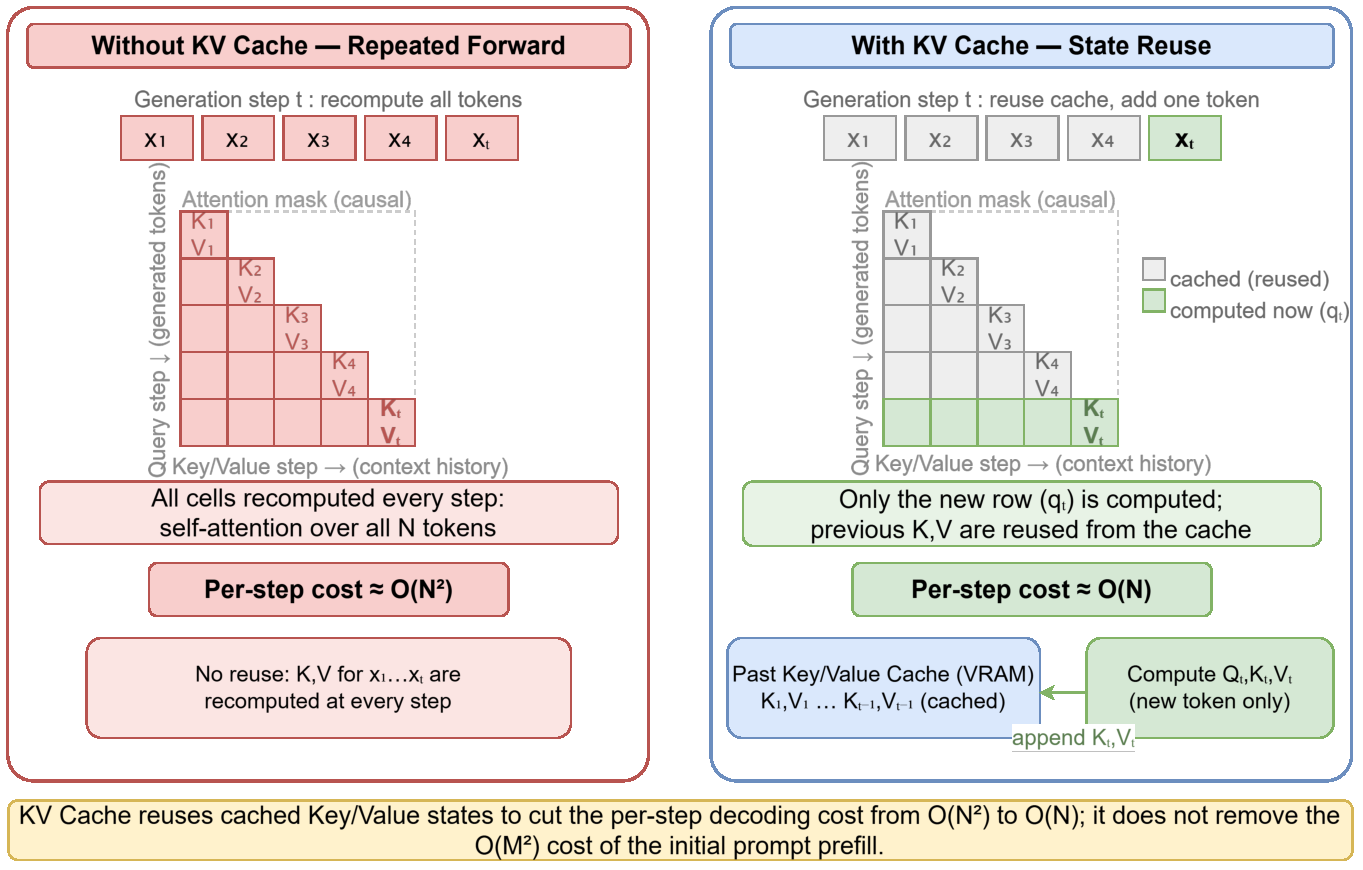
\includegraphics[width=0.85\textwidth]{Fig2.pdf}
\caption{Prompt-prefill scheduling. System A prefills the complete prompt after speech end; System B prefills committed fragments incrementally. Both systems use standard KV-cache reuse during autoregressive decoding.}
\label{fig:kvcache}
\end{figure*}

\subsection{Evaluation Metrics}

\subsubsection{Time to First Token and Time to First Audio}

TTFT follows Eq.~(\ref{eq:ttft}). In legacy prerecorded runs, $t_{\mathrm{speech\ end}}$ is the waveform feed-completion timestamp; in the unified TTFA run, all timestamps share one \texttt{perf\_counter\_ns} clock. TTFA follows Eq.~(\ref{eq:ttfa}), and ``playable'' means the first non-empty PCM accumulation of at least 1324 bytes. Its closed timeline is speech end $\rightarrow$ feed end $\rightarrow$ pipeline input close $\rightarrow$ first token $\rightarrow$ response text ready $\rightarrow$ TTS request $\rightarrow$ first playable PCM. We define
\begin{equation}
t_{\mathrm{feed\_to\_close\_wait}}=t_{\mathrm{input\ close}}-t_{\mathrm{feed\ end}}.
\label{eq:feedclose}
\end{equation}
This interval includes scheduling before and after explicit flush and must not be interpreted as flush computation alone.

\subsubsection{Recognition and Statistical Reporting}

Word error rate (WER), the standard metric for ASR accuracy, is computed from the Levenshtein edit distance:
\begin{equation}
\mathrm{WER}=\frac{S+D+I}{N_{\mathrm{ref}}}
\label{eq:wer}
\end{equation}

where $S$, $D$, and $I$ are substitution, deletion, and insertion counts and $N_{\mathrm{ref}}$ is the reference length. We primarily report WER for English and CER for Chinese. Table labels distinguish mean-utterance error (the arithmetic mean of sample-level rates) from corpus error $\sum(S+D+I)/\sum N_{\mathrm{ref}}$. Latency tables report the sample mean, sample standard deviation (\texttt{ddof}=1), and tail percentiles. Paired comparisons use 10,000 bootstrap resamples with seed 20260821 for percentile 95\% confidence intervals and two-sided Wilcoxon signed-rank tests; Holm correction is applied within the duration-group and augmentation families. Fig.~\ref{fig:trend} shows observed P5--P95 bands, not confidence intervals.

\section{System Design}\label{sec:design}

\subsection{Overall Architecture}

\subsubsection{Objective and Logical Topology}

The core design objective is to shift from the traditional ``receive everything, then process everything'' paradigm to an ``incremental receive, streaming process'' paradigm, driving first-token latency toward its theoretical lower bound. The logical topology is shown in Fig.~\ref{fig:topology}, which depicts the streaming parallel data flow built on multi-threaded producer--consumer queues. Audio enters the segmentation module continuously as fixed-length PCM chunks; Silero VAD performs activity detection on an accumulation buffer and emits speech segments~\cite{ref13}. The ASR module concatenates several speech segments, invokes Whisper for transcription, and emits append-only text fragments according to the prefix/suffix context policy. Text fragments are passed through a thread-safe queue to the LLM module, which keeps updating the KV cache and starts generation when the termination marker arrives, thereby moving as much LLM prefill computation as possible forward to overlap with audio input.

The overall architecture is a segment--transcribe--prefill--generate pipeline: as soon as an upstream module produces a new audio or text segment, the downstream module can start computing without waiting for the full input. The system comprises three subsystems: a Streaming Audio Segmenter for voice activity detection and segmentation, a Context-Aware ASR Engine for context concatenation and output stability, and an Incremental LLM Inference Service for incremental prefilling and final generation. The KV cache in the LLM part is a general optimization for Transformer decoder inference; we directly reuse the \texttt{past\_key\_values} mechanism built into the inference framework for state reuse.

\subsubsection{Key Engineering Details}

To keep the streaming pipeline real-time and controllable in a single-machine prototype, the implementation splits the chain into a multi-threaded pipeline decoupled by thread-safe queues, with state objects carrying cross-segment context.

For communication, modules do not call each other synchronously; they communicate asynchronously through a producer--consumer model. In the implementation, the audio-chunk queue, audio-segment queue, and text-segment queue are all instances of \texttt{queue.Queue}; consumers loop on \texttt{get} with a timeout, and a designated end-event marks the end of production, avoiding single-point blocking that could deadlock the pipeline. In the ASR stage, the system must simultaneously accept segmented audio from upstream and stream transcribed text downstream, so it is split into two sub-threads, a collector and a transcriber: the former continuously receives upstream speech segments and writes them to a waiting queue; the latter, when the trigger condition is met, concatenates them in batch, calls Whisper for transcription, and pushes the current commit region to the downstream LLM, decoupling audio collection from model inference.

\begin{figure*}[!t]
\centering
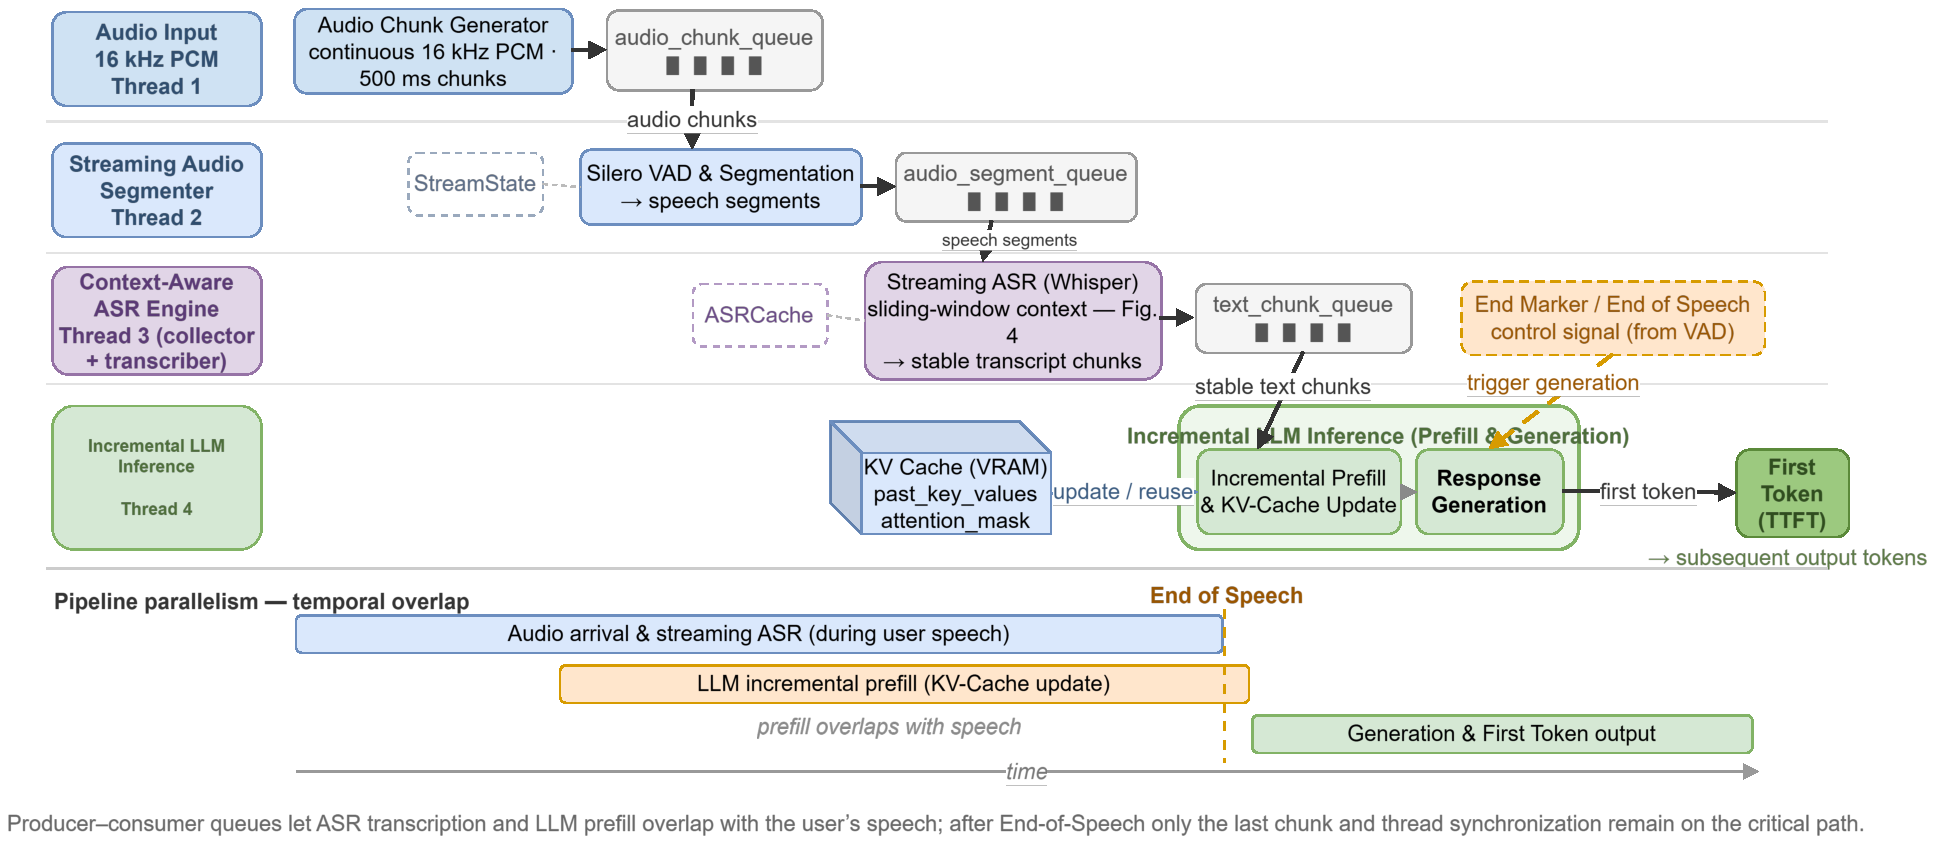
\includegraphics[width=\textwidth]{Fig3.pdf}
\caption{Logical topology of the streaming parallel architecture}
\label{fig:topology}
\end{figure*}

State management uses a hybrid stateful/stateless design. The segmentation module maintains the accumulated audio buffer, segment boundaries, and indices in \texttt{StreamState}. The ASR side manages pending and transcription-window queues in \texttt{ASRCache}. The LLM persists \texttt{past\_key\_values}, \texttt{attention\_mask}, and last-step prefill logits in \texttt{KVCache}. Together these objects maintain cross-segment state and an append-only downstream interface; they do not guarantee that later internal ASR hypotheses remain unchanged.

\subsection{Streaming ASR Context Management}\label{sec:asr-context}

\subsubsection{Strategy}

The central challenge of streaming ASR is balancing recognition accuracy against latency: slices that are too short deprive the model of necessary acoustic context and sharply increase the word error rate, while waiting for slices that are too long introduces significant buffering and processing delay, eroding the advantage of streaming. This section presents an adaptive context-management strategy based on a dynamic sliding window.

\subsubsection{Dynamic VAD Segmentation}

The system uses the Silero VAD model to segment the continuous PCM stream online. Define the input audio stream as a time series $\{x_1,x_2,\dots,x_t\}$. The segmenter maintains an accumulation buffer $A_{\mathrm{accum}}$ and, on receiving each new audio chunk $c_t$, performs $A_{\mathrm{accum}}\leftarrow A_{\mathrm{accum}}\oplus c_t$, where $\oplus$ denotes concatenation. Once the accumulated audio exceeds the minimum detection window, Silero VAD is invoked; if sufficiently long silence is detected and the speech segment exceeds the minimum speech threshold, the segment is considered closed and emitted to the downstream ASR. The prototype uses a 500~ms chunk length, a 2~s minimum speech length, and a 300~ms minimum silence duration. These values trade off responsiveness against segmentation stability: the 500~ms chunk gives fine online detection granularity while avoiding the frequent VAD calls and thread-scheduling overhead of shorter chunks; the 2~s minimum speech length ensures each fragment submitted to Whisper has enough context, reducing the instability of very short fragments; and the 300~ms silence threshold distinguishes intra-sentence pauses from true end of speech, preventing premature truncation. In terms of sensitivity, smaller chunks or silence thresholds shorten endpoint-detection waiting but may increase spurious segmentation and boundary jitter; larger chunks, minimum speech lengths, or silence thresholds improve stability but increase post-endpoint waiting. We therefore fix these VAD parameters in all comparison experiments to keep configurations comparable.

\subsubsection{Sliding-Window Context Awareness}

\begin{figure}[!t]
\centering
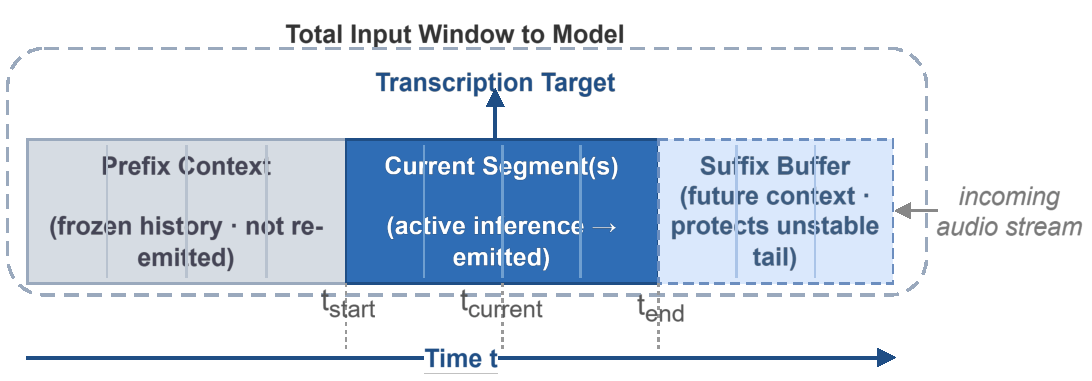
\includegraphics[width=\linewidth]{Fig4.pdf}
\caption{Schematic of the context-aware ASR sliding-window mechanism}
\label{fig:window}
\end{figure}

To reduce boundary effects in streaming recognition, the ASR engine uses a sliding window with prefix context. Fig.~\ref{fig:window} details the model input at time step $t$. The window contains frozen prefix audio, the target segment, and an optional suffix buffer. This overlap is intended to reduce boundary instability; it does not guarantee that later internal re-recognition will reproduce the same text.

First, the window is updated. Let $Q_t$ be the audio-segment queue at time $t$. Newly arrived segments first enter a waiting queue and are then merged in batch into the main queue by the transcription thread, yielding $Q_t$. Transcription is triggered when the accumulated queue duration reaches the threshold $\tau_{\mathrm{asr}}$ and the queue length satisfies (\ref{eq:trigger}):
\begin{equation}
\left|Q_{\mathrm{temp}}\right|\geq N_{\mathrm{prefix}}+1+N_{\mathrm{suffix}}
\label{eq:trigger}
\end{equation}

where $\left|Q_{\mathrm{temp}}\right|$ is the current temporary queue length and $N_{\mathrm{prefix}}$ and $N_{\mathrm{suffix}}$ are the configured numbers of preceding and following segments. When the condition is met, or when the final speech segment arrives, the ASR model concatenates all segments in the temporary queue and performs one transcription pass to produce the raw transcript. In practice a minimum-recognition threshold is also applied to avoid the frequent calls and unstable output caused by overly short windows.

Second, timestamp-aligned text extraction maps Whisper words to segment spans by word end time and emits only segments inside the current commit region. The first and final rounds receive explicit boundary handling so no trailing text is intentionally withheld. After emission, the window retains configured prefix and uncommitted suffix segments. A larger suffix can reduce some boundary errors but also delays commitment and adds decoding work; Table~\ref{tab:context} shows that its effect is metric- and language-dependent.

\subsubsection{Commit Contract and Tokenizer Seams}

The ASR maintains two state layers. Internal hypotheses may be overwritten when retained audio is recognized again. In contrast, a committed downstream fragment is delivered once and never retracted. There is no KV-cache rollback path: corrections observed internally after commitment are logged but are not propagated to the LLM. Thus ``append-only'' describes the downstream interface, not immutable internal recognition. A tokenizer seam occurs when fragment-wise tokenization differs from one-shot tokenization,
\begin{equation}
\mathcal{T}(f_1)\Vert\mathcal{T}(f_2)\neq\mathcal{T}(f_1\Vert f_2).
\label{eq:seam}
\end{equation}
The cache stores the actual fragment-wise token sequence. Measurements of internal drift and seam frequency are reported in Section~\ref{sec:stateeval}.

\subsection{Incremental KV-Cache Prefilling for the LLM}\label{sec:kv-prefill}

\subsubsection{Strategy}

In System~A, the LLM obtains the complete prompt only after ASR finishes transcribing the whole utterance, and performs prefill plus first-token generation entirely after the end-of-speech endpoint. TTFT therefore rises markedly as transcript length grows. Applying that serial paradigm unchanged to a setting where computation could proceed during audio input wastes the time window before the endpoint and squanders the available parallelism.

System~B reduces residual computation by retaining the \texttt{past\_key\_values} produced by each committed fragment. A new fragment triggers a forward pass only for its own tokens, after which the updated cache replaces the previous state. When input closes, any remaining fragment and the generation prompt are processed before decoding begins. The amount of work left at closure depends on the final segment and queue state; the design moves most, but not necessarily all, prefill into the speaking interval. Because the cache is append-only, revising an already delivered fragment would require rollback or recomputation, which this prototype does not implement.

\subsubsection{Core Algorithm}

The core logic of incremental inference: on the first call, the system performs a one-shot prefill without any cache, establishing the initial KV cache; thereafter, each new ASR text fragment from upstream triggers a call to \texttt{cache\_prompt()}, which updates incrementally on top of the existing \texttt{past\_key\_values}. When the termination marker is received, the system appends the generation prompt (e.g., ``assistant:'', telling the model that the next output token begins the assistant's reply) to the end of the prompt and reuses the last-step logits from prefilling to start decoding directly. To avoid positional-encoding misalignment of incremental tokens, the implementation constructs \texttt{position\_ids} explicitly and encodes new fragments without adding another generation prompt, keeping cache concatenation controlled. Algorithm~\ref{alg:prefill} gives the incremental update procedure corresponding to this implementation. Fig.~\ref{fig:kvupdate} visualizes the state changes in GPU memory: the blue region on the left is the cached key--value pairs of the historical context, and the green region on the right is the key--value pairs produced by the new fragment. On each fragment's arrival, incremental prefilling reuses the historical \texttt{past\_key\_values} and runs the forward pass only over new tokens before updating the cache, avoiding repeated prefills over the full prompt in the incremental setting.

\begin{algorithm}[!t]
\caption{Incremental KV cache prefill (StreamLLMInference)}\label{alg:prefill}
\begin{algorithmic}[1]
\Require current KV cache $C_{\mathrm{prev}}=(P_{\mathrm{prev}},\mathit{Mask}_{\mathrm{prev}},L_{\mathrm{prev}})$; new text fragment $T_{\mathrm{new}}$; end flag $\mathit{IsEnd}$; generation prompt $G$; tokenizer $\mathcal{T}$; LLM $\mathcal{M}$
\Ensure updated cache $C_{\mathrm{new}}=(P_{\mathrm{new}},\mathit{Mask}_{\mathrm{new}},L_{\mathrm{new}})$
\State \textbf{Step 1: fragment preparation and tokenization}
\If{$\mathit{IsEnd}=\mathrm{True}$}
    \State $T_{\mathrm{new}} \gets \mathrm{Concat}(T_{\mathrm{new}}, G)$ \Comment{append generation prompt}
\EndIf
\If{$T_{\mathrm{new}}$ is empty}
    \State \textbf{raise} exception \Comment{invalid empty fragment}
\EndIf
\State $\mathit{Ids}_{\mathrm{new}} \gets \mathcal{T}(T_{\mathrm{new}}, \texttt{add\_special\_tokens}=\mathrm{False})$
\If{$\mathit{Ids}_{\mathrm{new}}$ is empty}
    \State \textbf{raise} exception \Comment{no valid token in fragment}
\EndIf
\State \textbf{Step 2: attention mask and position IDs}
\State $\mathit{Mask}_{\mathrm{new}} \gets \mathrm{Concat}\left(\mathit{Mask}_{\mathrm{prev}},\,\mathbf{1}_{|\mathit{Ids}_{\mathrm{new}}|}\right)$
\State $\mathit{Pos} \gets \left[\,|\mathit{Mask}_{\mathrm{prev}}|,\dots,|\mathit{Mask}_{\mathrm{new}}|-1\,\right]$ \Comment{explicit \texttt{position\_ids}}
\State \textbf{Step 3: forward pass (incremental update)}
\State $\mathit{Outputs} \gets \mathcal{M}(\mathit{Ids}_{\mathrm{new}},\mathit{Mask}_{\mathrm{new}},\mathit{Pos},$
\Statex \hspace{\algorithmicindent} $P_{\mathrm{prev}},\texttt{use\_cache}=\mathrm{True})$
\Statex \hspace{\algorithmicindent} \Comment{forward only on new tokens, reusing cached $P_{\mathrm{prev}}$}
\State \textbf{Step 4: cache and logits update}
\State $P_{\mathrm{new}} \gets \mathit{Outputs}.\texttt{past\_key\_values}$
\State $L_{\mathrm{new}} \gets \mathit{Outputs}.\texttt{logits}[:, -1, :]$ \Comment{if $\mathit{IsEnd}=\mathrm{True}$, the first token is decoded from $L_{\mathrm{new}}$ without an extra forward pass}
\State $C_{\mathrm{new}} \gets (P_{\mathrm{new}},\mathit{Mask}_{\mathrm{new}},L_{\mathrm{new}})$
\State \Return $C_{\mathrm{new}}$
\end{algorithmic}
\end{algorithm}

\begin{figure}[!t]
\centering
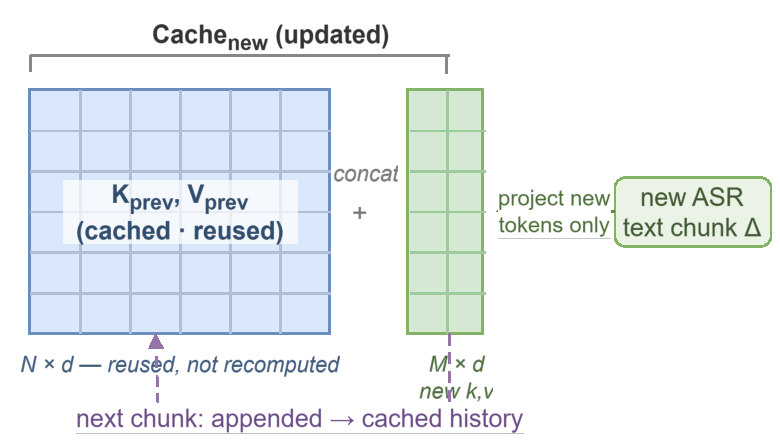
\includegraphics[width=\linewidth]{Fig5.pdf}
\caption{Schematic of the LLM KV Cache incremental update mechanism}
\label{fig:kvupdate}
\end{figure}

\subsubsection{Complexity Analysis}

To locate the source of the redundancy that incremental prefilling removes, consider one update with historical context length $N$ and new-fragment length $M$. If every incremental arrival triggered a fresh prefill over the whole sequence $x_{1:N+M}$ (no reuse of historical state), the dominant self-attention cost would be about $O\!\left((N+M)^{2}\right)$. With the KV cache, the $K,V$ of historical tokens are already stored; the system only computes queries for the new tokens and lets them interact with Key/Value of length $N+M$, at a dominant cost of $O\!\left(M(N+M)\right)$. When $M\ll N$ this approximates $O(MN)$, i.e., linear scaling in the new fragment. Note that if all incremental fragments accumulate to a final length $L$, the cumulative cost of incremental prefilling is
\begin{equation}
\sum_{j}O\!\left(M_j L_j\right)=O\!\left(L^{2}\right)
\label{eq:cumcost}
\end{equation}

where $M_j$ and $L_j$ are the length of the $j$-th new text fragment and the accumulated length, and $L$ is the full sequence length---the same order as offline one-shot prefilling. The key benefit of our strategy is not a lower complexity order but the relocation of prefill computation into the user's speaking time, so that the computation remaining after the end-of-speech endpoint consists mainly of the final small increment plus thread-synchronization overhead, effectively lowering TTFT. In addition, our implementation keeps the last-step \texttt{logits} of the prefill phase in the KV cache, so the first token can be decoded without any extra forward pass once the termination marker arrives, further trimming the constant overhead of the first-token phase.

\subsection{Test Data Construction Pipeline}\label{sec:data}

\subsubsection{Overview}

Systematically validating the streaming architecture under controlled conditions requires dialogue data of steadily increasing length, so we built an automated data-synthesis pipeline. It converts two standard multi-turn dialogue datasets, MultiWOZ (English)~\cite{ref14} and CrossWOZ (Chinese)~\cite{ref15}, into progressively lengthening long-speech test data with precise duration annotations, and then generates audio via TTS.

\subsubsection{Cumulative Dialogue Generation}

\begin{table*}[!t]
\caption{Dialogue data accumulation strategy (example translated from Chinese)}\label{tab:accum}
\centering
\begin{tabular}{@{}clll@{}}
\toprule
Turn & User & Agent & Accumulated text \\
\midrule
1 & Book a flight & Where to? & Book a flight \\
2 & \begin{tabular}[t]{@{}l@{}}To Beijing,\\ leaving tomorrow\end{tabular} & Which cabin class? & \begin{tabular}[t]{@{}l@{}}Book a flight, Where to?,\\ To Beijing, leaving tomorrow\end{tabular} \\
3 & Business class & OK, booking it now & \begin{tabular}[t]{@{}l@{}}Book a flight, Where to?, To Beijing, leaving\\ tomorrow. Which cabin class? Business class\end{tabular} \\
\bottomrule
\end{tabular}
\end{table*}

MultiWOZ and CrossWOZ both contain multi-turn dialogues, but individual user turns are usually short and cannot directly cover long-speech input. To simulate a user stating a complex request in one pass or continuously adding information, we construct long input samples with a cumulative dialogue strategy. As illustrated in Table~\ref{tab:accum}, the algorithm walks through the dialogue history turn by turn, concatenating the user-side inputs and system replies of the current and preceding turns into input sequences of increasing length.

This strategy generates continuous speech samples from 3 seconds to over 60 seconds grounded in real semantic context, covering interaction forms from short commands to extended statements and remedying the lack of long-speech samples in conventional datasets.

\subsubsection{Data Processing Pipeline}

Data construction proceeds in three strictly ordered stages.

The first is history accumulation and filtering. The strategy traverses the source datasets and applies the cumulative generation logic. To focus on long-speech bottlenecks, generated samples are sorted by text length in descending order and the longest $N$ dialogue fragments are selected first, with maximum text-length thresholds (2,050 characters for English, 720 for Chinese) to prevent out-of-memory errors; an upper bound on speech length also avoids needlessly inflating experiment time.

The second is concurrent TTS synthesis. We use Alibaba's CosyVoice service~\cite{ref17} to produce controlled synthetic waveforms from the accumulated text. A batch module issues asynchronous requests; the resulting audio remains synthetic and is not treated as human speech.

The third is duration calibration and metadata synchronization. Because generative TTS speaking rate is nondeterministic, estimating duration from character counts is error-prone. The pipeline parses the generated WAV file headers to obtain physical durations in seconds (accurate to milliseconds), which are written back to the test-metadata JSON as ground truth for the X-axis (input duration) of subsequent experiments.

\subsubsection{Test-Set Groups}

\begin{table*}[!t]
\caption{Audio duration groups}\label{tab:groups}
\centering
\begin{tabular}{@{}clll@{}}
\toprule
Group & Duration (s) & Typical scenario & Experimental focus \\
\midrule
Short & $T<5$ & Short commands & Baseline latency \\
Medium & $5\leq T<15$ & Multi-intent statements & Everyday dialogue performance \\
Long & $15\leq T<30$ & Complex long sentences & Core advantage region of streaming \\
Very Long & $30\leq T<60$ & Extended expositions & Tail-latency growth \\
Extra Long & $T\geq60$ & Extreme stress test & Stability and OOM boundary \\
\bottomrule
\end{tabular}
\end{table*}

For fine-grained analysis of latency across durations, the generated samples are divided into five standard groups by audio duration (Table~\ref{tab:groups}).

This grouping is used throughout the experimental analysis in Section~\ref{sec:experiments} to compare how the architectures handle speech of different lengths.

\subsubsection{Concatenated Human-Read Speech and Augmentation}

To test acoustic conditions not represented by TTS, we construct long-form samples from LibriSpeech test-clean~\cite{panayotov2015librispeech} and AISHELL-1~\cite{bu2017aishell1}. LibriSpeech utterances are concatenated in chapter order and AISHELL-1 utterances in speaker order. Uniformly sampled silences $U(0.2,1.0)$~s are inserted between source utterances with seed 42. Each language contributes 75 clean samples (30 Long, 30 Very Long, and 15 Extra Long), adding multiple speakers and recording conditions; AISHELL-1 further broadens Mandarin speaker and accent coverage. For each language, six 30-sample variants add MUSAN~\cite{snyder2015musan} noise at SNR 20, 15, and 10~dB, apply speed factors 0.9 and 1.1, or add 15-dB babble. Speed-modified samples are regrouped using their new durations. A five-sample manual listening check passed intelligibility and alignment checks, while confirming that concatenation seams can be audible. We therefore describe these data as concatenated human-read speech rather than spontaneous dialogue.

\section{Experiments and Analysis}\label{sec:experiments}

\subsection{Experimental Protocol}

System~A is a serial non-streaming cascade: full-audio Whisper transcription is followed by one-shot Qwen2-7B-Instruct~\cite{ref20} prompt prefill and generation. System~B uses the same weights but applies the streaming ASR and incremental prefill mechanisms described above. Tables~\ref{tab:ttft}--\ref{tab:context} and Fig.~\ref{fig:trend} use the original 2025 dual-RTX~3090 platform. Repeated measurements and Tables~\ref{tab:real}--\ref{tab:ttfa} use a second platform, a KVM virtual machine with an Intel Xeon Gold 6133 at 2.50~GHz and two RTX~3090 GPUs. Absolute latency is platform-dependent, so values from the two platforms are neither scaled nor mixed within a comparison. In both environments, Whisper-Turbo runs on one GPU and Qwen2-7B-Instruct on the other, batch size is one, and three real-audio warm-up runs precede measurement.

Tables~\ref{tab:ttft}--\ref{tab:context} use a 50-token generation cap. The state, semantic, and unified TTFA experiments use 128 tokens. Effective sampling uses temperature 0.1 and top-$p$ 0.9. Although the historical interface accepted \texttt{repetition\_penalty=1.1}, post-experiment inspection found that the custom decoder did not apply it; all compared arms therefore used no effective repetition penalty. The original-platform mixed synthetic set contains 1,132 samples: 630 from MultiWOZ and 502 from CrossWOZ. Paired exclusions are stated with each experiment.

\subsection{Latency versus Speech Length}

\begin{figure}[!t]
\centering
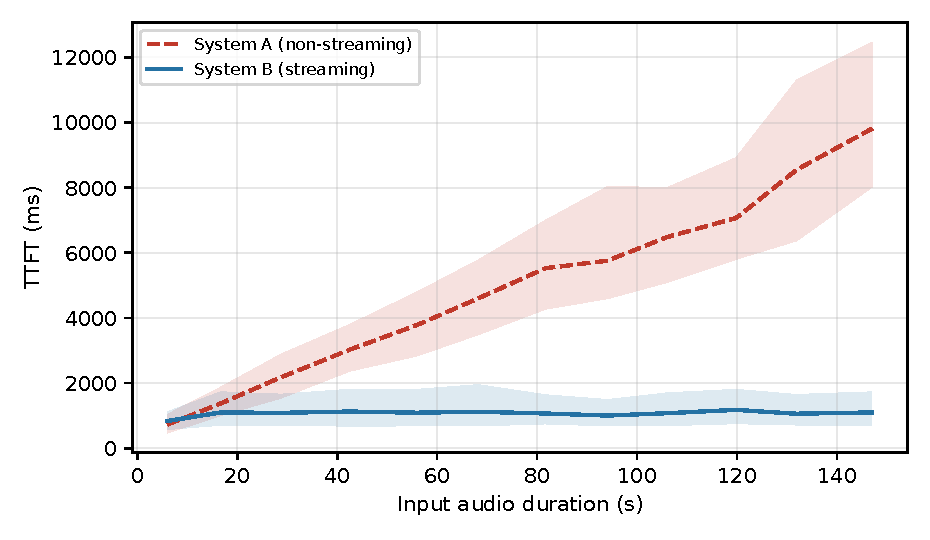
\includegraphics[width=\linewidth]{Fig6.pdf}
\caption{TTFT over 12 equal-frequency duration bins. Lines show bin means and shaded regions show observed P5--P95 ranges, not confidence intervals.}
\label{fig:trend}
\end{figure}

\begin{table*}[!t]
\caption{TTFT by duration on the original platform (ms)}\label{tab:ttft}
\centering
\scriptsize
\begin{tabular}{@{}lrrrrrrr@{}}
\toprule
Group & $n$ & \multicolumn{3}{c}{System B} & \multicolumn{3}{c}{System A} \\
\cmidrule(lr){3-5}\cmidrule(l){6-8}
& & Mean$\pm$std & P95 & P99 & Mean$\pm$std & P95 & P99 \\
\midrule
Short & 35 & 648.17$\pm$70.76 & 744.76 & 797.17 & 533.42$\pm$65.44 & 631.82 & 674.06 \\
Medium & 89 & 959.53$\pm$184.10 & 1261.82 & 1397.39 & 923.42$\pm$170.86 & 1196.04 & 1281.49 \\
Long & 121 & 1126.63$\pm$323.72 & 1883.55 & 1978.67 & 1722.04$\pm$342.63 & 2310.40 & 2474.07 \\
Very Long & 208 & 1099.16$\pm$343.51 & 1768.83 & 2173.97 & 3191.97$\pm$697.81 & 4467.14 & 4826.85 \\
Extra Long & 679 & 1087.70$\pm$383.16 & 1717.10 & 2605.45 & 6745.57$\pm$2108.79 & 11313.22 & 12274.38 \\
\bottomrule
\end{tabular}
\end{table*}

System~B adds fixed overhead for Short and Medium samples, but its mean TTFT changes little over the three longer groups on the original platform. For Long, Very Long, and Extra Long input, mean reductions are 34.6\%, 65.6\%, and 83.9\%; paired bootstrap 95\% confidence intervals for the reduction are [30.6\%, 38.3\%], [63.8\%, 67.3\%], and [83.3\%, 84.4\%], respectively, with Holm-adjusted Wilcoxon $p<2.1\times10^{-19}$. The Extra Long absolute reduction is 5657.9~ms (5.66~s). Tail latency is not constant: System~B P99 rises from 1978.67 to 2605.45~ms between Long and Extra Long. This 1.32$\times$ growth is nevertheless smaller than System~A's 4.96$\times$ growth, and the Extra Long P99 is 0.21$\times$ the baseline value. The empirical crossover depends on platform and speech distribution; the 15-s group boundary is not asserted as a universal routing threshold.

\subsubsection{Repeated Measurements}

On the second platform, 50 fixed Very Long samples were run three times per mode. System~B round means were 1434.0, 1482.1, and 1454.9~ms, a range equal to 3.3\% of the grand mean; System~A means were 4063.3, 4244.2, and 4118.5~ms. With sample standard deviation, System~B per-sample coefficient of variation (CV) had mean 5.19\%, median 4.05\%, P90 10.73\%, and maximum 18.96\%; the corresponding System~A values were 5.23\%, 4.65\%, 9.92\%, and 14.01\%. Central behavior was repeatable, but both modes retained a non-negligible high-variance tail.

\subsection{Ablation and Context Trade-offs}

The ablation starts from 505 Long-or-longer candidates. Pairwise exclusion removes three runtime errors and four cases in which a streaming arm exceeded 10~s, leaving 498 samples (108 Long, 150 Very Long, and 240 Extra Long). The unfiltered failure/hang rate is therefore 7/505 (1.4\%).

\begin{table*}[!t]
\caption{Ablation on the original platform; cells are mean$\pm$std [P95/P99] ms}\label{tab:ablation}
\centering
\scriptsize
\begin{tabular}{@{}lccc rr@{}}
\toprule
Group & Baseline & Streaming ASR only & Full streaming & ASR gain & KV gain \\
\midrule
Long & 1690.81$\pm$349.51 [2323.60/2431.03] & 1064.67$\pm$307.62 [1691.03/1873.56] & 1087.69$\pm$312.46 [1748.08/1859.16] & 626.13 & $-23.01$ \\
Very Long & 3307.96$\pm$872.57 [4891.94/5468.95] & 1155.09$\pm$365.67 [1859.20/2259.80] & 1152.36$\pm$363.23 [1828.80/2228.55] & 2152.87 & 2.73 \\
Extra Long & 6515.67$\pm$1762.26 [9208.54/9619.23] & 1228.82$\pm$411.10 [1981.51/2858.89] & 1188.00$\pm$411.07 [1946.51/2812.95] & 5286.86 & 40.82 \\
\bottomrule
\end{tabular}
\end{table*}

Streaming ASR is the dominant source of measured reduction: its gains are 626.13, 2152.87, and 5286.86~ms. Incremental prefill has no monotonic independent effect across the groups: $-23.01$, 2.73, and 40.82~ms relative to Streaming ASR Only. The Extra Long value is 3.3\% of the ASR-only TTFT. Thus incremental prefill remains an architectural mechanism for moving prompt work before speech end, but its isolated marginal TTFT effect is small for Qwen2-7B on this platform.

\begin{table*}[!t]
\caption{Context-window accuracy and pooled ASR time on the original platform; cells show mean$\pm$std [P95/P99]}\label{tab:context}
\centering
\scriptsize
\setlength{\tabcolsep}{3pt}
\begin{tabular}{@{}lccccc@{}}
\toprule
Configuration & MultiWOZ WER & MultiWOZ CER & CrossWOZ WER & CrossWOZ CER & Pooled ASR time (ms) \\
\midrule
Prefix 1 + suffix 1 & .0895$\pm$.0614 [.1960/.2482] & .0196$\pm$.0208 [.0611/.0799] & .0083$\pm$.0160 [.0431/.0659] & .0203$\pm$.0276 [.0747/.1054] & 1327.48$\pm$645.03 [2716.80/3049.16] \\
Prefix 1 + suffix 0 & .0813$\pm$.0611 [.1882/.2465] & .0221$\pm$.0218 [.0603/.0842] & .0118$\pm$.0188 [.0482/.0723] & .0292$\pm$.0339 [.0927/.1193] & 1224.96$\pm$655.85 [2726.57/3018.06] \\
Prefix 0 + suffix 0 & .0619$\pm$.0678 [.1756/.3086] & .0226$\pm$.0265 [.0657/.1072] & .0210$\pm$.0237 [.0633/.0870] & .0500$\pm$.0374 [.1146/.1316] & 1086.16$\pm$690.43 [2641.87/2973.93] \\
\bottomrule
\end{tabular}
\end{table*}

Each context configuration contains 74 MultiWOZ and 76 CrossWOZ samples. Error cells are mean-utterance metrics; the ASR time column pools the streaming and non-streaming records ($n=300$) and is not interpreted as streaming tail latency alone. Adding one suffix segment reduces CrossWOZ WER/CER from 0.0118/0.0292 to 0.0083/0.0203 while increasing pooled ASR time. Removing all extra context is faster but raises CrossWOZ WER/CER to 0.0210/0.0500. MultiWOZ WER is not monotonic in context size. These data establish a measured trade-off on synthetic speech, not a universal language-specific configuration rule. System~A's near-zero error in this experiment is specific to TTS generated from its reference text.

\subsection{Concatenated Human-Read Speech}\label{sec:realexp}

\begin{table*}[!t]
\caption{Concatenated human-read speech and augmentation results on the second platform}\label{tab:real}
\centering
\scriptsize
\begin{tabular}{@{}llrrrr@{}}
\toprule
Language & Condition ($n$) & A TTFT & B TTFT & A error & B error \\
\midrule
English & Clean (75) & 2805.9 & 1672.1 & .0297 [.0290] & .0565 [.0499] \\
English & SNR 20 dB (30) & 2228.8 & 1633.1 & .0288 [.0270] & .0627 [.0573] \\
English & SNR 15 dB (30) & 2334.3 & 1801.5 & .0255 [.0264] & .0578 [.0556] \\
English & SNR 10 dB (30) & 2201.4 & 1654.3 & .0372 [.0387] & .0817 [.0799] \\
English & Speed 0.9$\times$ (30) & 2341.8 & 1602.4 & .0458 [.0491] & .0751 [.0751] \\
English & Speed 1.1$\times$ (30) & 2181.7 & 1657.0 & .0380 [.0440] & .0741 [.0767] \\
English & Babble (30) & 2325.8 & 3425.1 & .0271 [.0296] & .4372 [.4001] \\
\midrule
Chinese & Clean (75) & 2871.7 & 1698.8 & .1077 [.1118] & .1180 [.1255] \\
Chinese & SNR 20 dB (30) & 2294.6 & 1696.1 & .1224 [.1281] & .1242 [.1299] \\
Chinese & SNR 15 dB (30) & 2290.5 & 1630.6 & .1064 [.1137] & .1110 [.1173] \\
Chinese & SNR 10 dB (30) & 2311.8 & 1654.7 & .1233 [.1275] & .1312 [.1405] \\
Chinese & Speed 0.9$\times$ (30) & 2236.5 & 1539.1 & .1232 [.1306] & .1380 [.1392] \\
Chinese & Speed 1.1$\times$ (30) & 2125.4 & 1623.6 & .1510 [.1612] & .1827 [.1918] \\
Chinese & Babble (30) & 2227.7 & 2082.2 & .1360 [.1429] & .2863 [.2662] \\
\bottomrule
\multicolumn{6}{l}{\footnotesize TTFT is mean ms. Error is mean-utterance [corpus] WER for English and CER for Chinese.}
\end{tabular}
\end{table*}

On clean LibriSpeech, Extra Long mean TTFT is 4805.1$\pm$420.2~ms for System~A and 1559.0$\pm$490.3~ms for System~B, a 67.5\% reduction. On clean AISHELL-1 the corresponding values are 5139.9$\pm$381.7 and 1762.9$\pm$275.4~ms, a 65.7\% reduction. The clean human-read System~A errors are no longer near zero: mean-utterance WER is 2.97\% on LibriSpeech and CER is 10.77\% on AISHELL-1; System~B obtains 5.65\% and 11.80\%. AISHELL-1 references spell numbers in Chinese while Whisper often emits Arabic numerals; this affects 49/75 clean samples (mean CER 0.1476 when affected versus 0.0313 otherwise).

Across the ten SNR and speed conditions, TTFT reduction ranges from 22.8\% to 31.6\%, with Holm-adjusted paired tests at $p\leq0.0129$. Babble is a boundary rather than a success case. For English, System~B is 47.3\% slower in the unpaired overall summary; paired inference on 29 common samples has a confidence interval reaching zero. Chinese babble yields only a 6.5\% mean reduction and is not significant ($p=0.271$). VAD over-triggering creates segment backlog, while Whisper produces empty streaming outputs for 12/30 English and 5/30 Chinese samples. English-babble System~B has median 2020.4~ms but mean 3425.1~ms, and the slowest sample takes approximately 21~s after audio completion to drain the ASR queue.

\subsection{Matched Streaming Baseline}

We implement a project-internal LocalAgreement-2-style baseline following the partial-hypothesis policy of Liu et al.~\cite{liu2020partialhypothesis} and its Whisper adaptation~\cite{machacek2023turning}. It uses the same Whisper weights, inference engine, and segmentation as System~B, with absolute-time-axis commitment, punctuation-robust agreement, sentence-boundary-aware trimming, and a 15-s retained-buffer cap. All three systems are rerun on the same second-platform 498-sample paired subset, and only the final validated baseline implementation is included.

\begin{table*}[!t]
\caption{Matched baseline comparison on the second platform}\label{tab:la}
\centering
\scriptsize
\begin{tabular}{@{}lrrrrrrrr@{}}
\toprule
System & Overall TTFT & P50 & P95 & Long & Very Long & Extra Long & zh CER & en WER \\
\midrule
System A & 5310.8$\pm$2817.9 & 4780.9 & 10462.1 & 1958.2 & 3905.9 & 7697.5 & .0674 & .1527 \\
System B & 1573.9$\pm$411.6 & 1484.4 & 2296.5 & 1464.3 & 1551.1 & 1637.5 & .0732 & .1702 \\
LA-2-style & 2115.0$\pm$693.3 & 1948.5 & 3463.2 & 1741.0 & 2199.7 & 2230.4 & .0835 & .1566 \\
\bottomrule
\multicolumn{9}{l}{\footnotesize TTFT values are ms; error values are mean-utterance metrics. Overall WER: A .0951, B .1047, LA .1073.}
\end{tabular}
\end{table*}

The LA-style baseline is approximately 34\% slower than System~B (2115.0 versus 1573.9~ms). The paired mean difference is 541.1~ms, with bootstrap 95\% CI [485.3, 599.9] and Wilcoxon $p=1.24\times10^{-70}$. Recognition errors remain of the same order, which supports latency attribution but does not establish statistical quality equivalence. Repeated whole-buffer decoding also degrades more on longer input: LA-style TTFT is 2199.7--2230.4~ms for Very Long and Extra Long samples, compared with 1551.1--1637.5~ms for System~B.

\subsection{Commitment, Tokenizer Seams, and Semantics}\label{sec:stateeval}

Instrumentation on 50 fixed Very Long synthetic samples records 375 downstream commits and zero rollback deliveries. Internal re-recognition nevertheless changes previously committed-region hypotheses 224 times, affecting 224/425 committed segments (52.7\%) and 49/50 samples. Character edit distance has mean 2.3, P90 6, and maximum 16; normalized edit ratio has mean 5.6\% and maximum 47.1\%. The changes include lexical drift but remain invisible to downstream consumers. Concatenated System~B text differs from System~A full transcription by mean WER 4.93\% and CER 2.69\%.

Fragment-wise and one-shot token sequences differ at seams in 25/50 samples, with means of 4.36 differing blocks and 5.60 one-shot-side tokens among affected samples. Decoding both token sequences reconstructs identical text in all 50 cases. This supports text-level reconstruction only; it does not establish token, KV-state, or output-distribution equivalence.

Response quality is explored on the same 25 Chinese and 25 English synthetic samples. Replies are independently sampled with the 128-token cap. BGE-M3~\cite{chen2024m3embedding} CLS embeddings with L2-normalized cosine yield mean 0.8832$\pm$0.0755 (minimum 0.6232, P10 0.7951). A paired-equivalence judge gives 2.96/5 and 40.0\% at or above 4; this measure confounds independent recommendation choices and truncation. A separate blinded intent-satisfaction judge gives System~A 3.10/5 and System~B 3.04/5; the paired B$-$A difference is $-0.06$ with bootstrap 95\% CI [$-0.34$, 0.22]. The judge is the Command Code service model \texttt{deepseek/deepseek-v4-flash}~\cite{commandcode2026deepseekv4flash}, temperature 0, with deterministic A/B order randomization. This single-judge, 50-sample analysis is exploratory and is not an equivalence claim.

\subsection{Unified Time to First Audio}

Table~\ref{tab:ttfa} uses only the R7 unified run on the second platform. Each mode has 25 Chinese and 25 English samples on one monotonic clock. System~B sends the first completed sentence to TTS, whereas System~A follows its non-streaming full-response text path; this is an end-to-end system-policy comparison, not an isolated TTS comparison with identical text. The local ASR/LLM pipeline uses in-process queues and TTS runs on localhost.

\begin{table*}[!t]
\caption{Unified TTFA and component decomposition on the second platform (ms)}\label{tab:ttfa}
\centering
\scriptsize
\begin{tabular}{@{}llrrrrr@{}}
\toprule
System & Language & Mean$\pm$std & P50 & P90 & P95 & $n$ \\
\midrule
System B & Chinese & 3303.3$\pm$2681.3 & 2603.0 & 3130.4 & 8299.2 & 25 \\
System B & English & 7660.5$\pm$2781.2 & 7577.0 & 10940.4 & 11857.2 & 25 \\
System B & All & 5481.9$\pm$3486.1 & 3113.7 & 10506.6 & 11656.3 & 50 \\
System A & Chinese & 22616.8$\pm$2197.2 & 22161.4 & 25459.9 & 26874.8 & 25 \\
System A & English & 22234.7$\pm$2850.4 & 22439.6 & 25274.4 & 26487.5 & 25 \\
System A & All & 22425.7$\pm$2526.1 & 22269.9 & 25588.8 & 26887.4 & 50 \\
\midrule
\multicolumn{7}{c}{Component means$\pm$std for all languages} \\
\midrule
\multicolumn{2}{l}{Component} & \multicolumn{2}{c}{System B} & \multicolumn{2}{c}{System A} & \\
\cmidrule(lr){3-4}\cmidrule(lr){5-6}
\multicolumn{2}{l}{Speech end $\rightarrow$ feed end} & \multicolumn{2}{c}{0.1$\pm$0.0} & \multicolumn{2}{c}{0.1$\pm$0.0} & \\
\multicolumn{2}{l}{Feed end $\rightarrow$ input close} & \multicolumn{2}{c}{133.0$\pm$98.7} & \multicolumn{2}{c}{0.0$\pm$0.0} & \\
\multicolumn{2}{l}{Input close $\rightarrow$ first token} & \multicolumn{2}{c}{1383.1$\pm$278.8} & \multicolumn{2}{c}{4182.9$\pm$898.3} & \\
\multicolumn{2}{l}{First token $\rightarrow$ text ready} & \multicolumn{2}{c}{387.0$\pm$429.2} & \multicolumn{2}{c}{4681.1$\pm$583.9} & \\
\multicolumn{2}{l}{Text ready $\rightarrow$ TTS request} & \multicolumn{2}{c}{0.4$\pm$0.1} & \multicolumn{2}{c}{0.6$\pm$0.1} & \\
\multicolumn{2}{l}{TTS request $\rightarrow$ playable PCM} & \multicolumn{2}{c}{3578.3$\pm$3023.6} & \multicolumn{2}{c}{13561.1$\pm$2513.6} & \\
\multicolumn{2}{l}{Closed sum} & \multicolumn{2}{c}{5481.9} & \multicolumn{2}{c}{22425.7} & \\
\bottomrule
\end{tabular}
\end{table*}

System~B reduces median TTFA by 86.0\%, from 22269.9 to 3113.7~ms. TTS remains the largest mean component and is highly variable, especially for English. The six components close exactly for all 100 records. The 133.0-ms $t_{\mathrm{feed\_to\_close\_wait}}$ is the complete feed-end-to-input-close interval; independent audit attributes approximately 132.68~ms to waiting before explicit flush, 0.21~ms to explicit flush, and 0.12~ms after flush. It is therefore not a flush-computation cost. On a ten-sample three-round subset, TTFA CV has mean 7.73\% and maximum 20.70\%. The 128-token cap affects both arms: 84/100 responses terminate at the cap and 16 by EOS.

\section{Conclusion and Outlook}\label{sec:conclusion}

\subsection{Summary}

This paper presents a pipeline-parallel cascade that moves chunked ASR and LLM prompt prefilling into the user's speaking interval. The design preserves the existing Whisper and Qwen2 weights and does not change the asymptotic attention cost; it changes scheduling and state reuse. On the same 498-sample synthetic subset, the overall TTFT reduction is 74.3\% on the original platform and 70.4\% on the second platform. On the original platform, mean System~B TTFT remains near 1.1~s from Long through Extra Long, while P99 grows only 1.32$\times$ compared with 4.96$\times$ for System~A. Concatenated human-read speech reproduces the Extra Long advantage, with reductions of 67.5\% on LibriSpeech and 65.7\% on AISHELL-1. Ablation shows that streaming ASR supplies most of the measured gain; the independent incremental-prefill effect is small under Qwen2-7B. The matched LA-style baseline is approximately 34\% slower than System~B. Unified measurement further reduces median TTFA from 22.27 to 3.11~s.

The implementation provides an append-only downstream text contract rather than immutable internal recognition. Internal hypotheses drift in the instrumented subset, tokenizer seams change token segmentation in half the samples, and the limited semantic experiment does not establish equivalence. These findings bound the claim: the architecture substantially weakens the growth of post-speech latency over the tested range while exposing concrete recognition, scheduling, and synthesis trade-offs.

\subsection{Limitations}

The main 1,132-sample benchmark remains TTS-synthesized. The added LibriSpeech/AISHELL-1 data are concatenated human-read utterances, not spontaneous dialogue, and some concatenation seams are audible. Babble noise is a demonstrated failure boundary because VAD over-triggering and empty ASR outputs create backlog and long tails. Experiments use exclusive GPUs, a single-machine ASR/LLM queue topology, and localhost TTS; distributed network latency and GPU contention are not represented, and absolute TTFT is CPU- and platform-sensitive.

The downstream interface never rolls back text, but internal re-recognition frequently changes committed-region hypotheses. Fragment-wise tokenization also differs from one-shot tokenization, so KV-state equivalence is not established. Semantic evidence covers only 50 Very Long synthetic samples, independently sampled replies, a 128-token cap, and one service judge without repeated ratings. The unified TTFA experiment uses sentence-ready System~B output versus the non-streaming System~A response path, and TTS contributes a large language-dependent tail. Finally, the prototype remains half-duplex and loses paralinguistic information at the text interface~\cite{ref22}.

\subsection{Future Work}

Future work should evaluate spontaneous, accented, microphone, and overlapping speech; add VAD back-pressure and adaptive segmentation for babble; and test task completion with repeated human and multi-judge assessment. Rollback-aware cache repair or retokenization could reconcile later ASR corrections and tokenizer seams. Platform-aware routing should replace a fixed duration threshold. Lower-latency incremental TTS, distributed deployment measurements, GPU-contention tests, larger LLMs, and full-duplex interruption handling would clarify how the observed scheduling gains transfer to production systems.

\section*{Acknowledgment}

The authors thank the School of Computer, Electronics and Information, Guangxi University, for providing the research environment that supported this work. The authors gratefully acknowledge the open-source projects that made this work possible, including OpenAI Whisper, Silero VAD, and CosyVoice. The authors also thank the anonymous reviewers for their constructive comments.

\bibliographystyle{IEEEtran}
\bibliography{refs}

\end{document}
